% !TEX root = ../thesis.tex
\section{Akustické modelování}
\label{chap:asr:acoustic}

Akustický model (AM) je v~rovnici (\ref{eq:asr:decoding:generic}) reprezentován podmíněnou pravděpodobností $P(\boldsymbol{O}|W)$. Úkolem akustického modelu je poskytnout co nejpřesnější odhad této pravděpodobnosti pro libovolnou posloupnost vektorů příznaků $\boldsymbol{O} = \left\{\boldsymbol{o}_1, \boldsymbol{o}_2\ \dots\ \boldsymbol{o}_T\right\}$. Jako velmi vhodný nástroj pro modelování řeči se ukázaly tzv. \textbf{skryté Markovovy modely (HMM)}. Ty vycházejí z principu vytváření řeči člověkem. V~průběhu produkce řeči se hlasové ústrojí v~krátkém časovém úseku nachází v~určité konfiguraci, přičemž množina všech možných konfigurací je konečná. Ve zvoleném krátkém úseku řeči (mikrosegmentu) je pak hlasovým ústrojím generován signál, který závisí na aktuální konfiguraci hlasového ústrojí. Tento vyprodukovaný zvuk je pomocí metod popsaných v~části \ref{chap:asr:parametrization} převeden na vektor příznaků $\boldsymbol{O}$.

Skrytý Markovův model je model stochastického procesu. Na ten je možné nahlížet jako na pravděpodobnostní konečný automat, který v~diskrétních časových okamžicích generuje náhodnou posloupnost vektorů příznaků $\boldsymbol{O} = \left\{\boldsymbol{o}_1, \boldsymbol{o}_2\ \dots\ \boldsymbol{o}_T\right\}$. Model v~každém časovém kroku změní stav svůj $s_j$ podle předem daných pravděpodobností přechodu $a_{ij}$. Přechod ze stavu $s_i$ do stavu $s_j$ má za následek vygenerování výstupního vektoru pozorování $\boldsymbol{o}_t$, a to podle rozdělení výstupní pravděpodobnosti $b_j\left(\boldsymbol{o}_t\right)$ příslušné  k~tomuto stavu \cite{Psutka2006}.

Podmíněná pravděpodobnost přechodu $a_{ij}$ určuje, s~jakou pravděpodobností přechází model ze stavu $i$ v~čase $t$, do stavu $j$ v~čase $t+1$. Platí tedy

\begin{equation}
  a_{ij} = p\left(s\left(t+1\right)=s_j|s\left(t\right)=s_i\right),
  \label{eq:asr:acoustic:conditional}
\end{equation}

\noindent kde $s\left(t\right)$ je stav modelu v~čase $t$. Další podmínkou je, že pro všechny stavy $i$, $i=1,2,\dots\,N$, platí

\begin{equation}
  \sum_{j=1}^{N} a_{ij} = 1.
  \label{eq:asr:acoustic:state:condition}
\end{equation}

\noindent Funkce rozdělení výstupní pravděpodobnosti $b_j\left(\boldsymbol{o}_t\right)$ popisují rozdělení pravděpodobnosti pozorování $\boldsymbol{o}_t$ produkovaného ve stavu $s_j$ v~čase $t$. Pro tuto funkci platí

\begin{equation}
  b_j\left(\boldsymbol{o}_t\right) = P\left(\boldsymbol{o}_t|s\left(t\right)=s\right),
  \label{eq:asr:acoustic:state:output}
\end{equation}

\noindent kde $P$ značí pravděpodobnost, pro kterou u spojitého rozdělení platí

\begin{equation}
  \int_{\boldsymbol{o}} b_j\left(\boldsymbol{o}\right)d\boldsymbol{o} = 1,
  \label{eq:asr:acoustic:state:output:condition:continous}
\end{equation}

\noindent kde toto platí pro všechny stavy HMM, které mohou generovat výstupní vektor.

% \noindent kde $P$ značí pravděpodobnost, pro kterou u diskrétních rozdělení platí

% \begin{equation}
%   \sum_o b_j\left(o\right) = 1.
%   \label{eq:asr:acoustic:state:output:condition:discrete}
% \end{equation}

% \noindent Pro spojité rozdělení pak alternativně

% \begin{equation}
%   \int_o b_j\left(o\right)do = 1.
%   \label{eq:asr:acoustic:state:output:condition:continous}
% \end{equation}

% \noindent v~obou případech to platí pro všechny stavy HMM, které mohou generovat výstupní vektor.

Rozdělení výstupní pravděpodobnosti musí být při modelování řečových zvuků dostatečně specifické, aby bylo možné od sebe odlišit různé zvuky, a zároveň dostatečně robustní, aby zahrnulo značnou variabilitu řečového signálu. Toto rozdělení je nejčastěji modelováno dvěma postupy, a to

\begin{itemize}
  \item spojitým normálním rozdělením se směsí hustotních funkcí,
  \item neuronovými sítěmi.
\end{itemize}

\subsection{Struktura skrytého Markovova modelu}
\label{chap:asr:acoustic:HMM}

Z pohledu rozpoznávání řeči se nejčastěji využívá tzv. levo-pravá struktura Markovova modelu. V~průběhu let bylo testováno mnoho různých struktur HMM, např. modely s~počtem stavů odvozených od průměrné délky slova, pro kterou byl model konstruován, až po pevnou strukturu stavů pro každé slovo. Tyto modely sloužily hlavně pro rozpoznávání izolovaných úseků řeči, nejčastěji slov.

Zatímco v~minulosti byly systémy rozpoznávání řeči založené na modelech celých slov, v~současnosti jsou pro zpracování kontinuální řeči využívány systémy pracující s~modely odvozenými od menších jednotek než jsou slova.
%V současnosti, kdy je většina systémů konstruovaných pro zpracování souvislé řeči a počet slov ve slovníku může přesahovat 1 milion slov, převažují modely odvozené od menších jednotek, než jsou slova.
Takovými jednotkami mohou být například fonémy anebo specifičtější trifóny. Trifón je svým způsobem kontextově závislý foném, který bere v~potaz svůj levý a pravý kontext, tj. levý a pravý sousední foném. Přepis slova do fonémové, resp. trifónové struktury lze ukázat na příkladu izolovaného slova \uv{akcie}, které má přepis \uv{\texttt{sil a  k~c i j e sil}}, v~trifónové podobě je pak zápis následující

\begin{verbatim}
  sil sil-a+k a-k+c k-c+i c-i+j i-j+e j-e+sil sil,
\end{verbatim}

\noindent kde \texttt{sil} má význam pauzy před, případně za vyslovenou promluvou slova \uv{akcie}.

Oproti slovním modelům, u fonémů (monofónů), resp. trifónů bývá struktura relativně jednoduchá a často je vyjádřena pětistavovým modelem, jehož podoba je přiblížena na obr. \ref{fig:asr:acoustic:hmm}. Jedná se o pětistavový levo-pravý Markovův model, jehož první a poslední stav jsou tzv. neemitující. Jejich primární úlohou je zřetězování jednotlivých HMM modelů trifónů (monofónů) do rozsáhlejších modelů, např. slov nebo vět. Při zřetězení se tyto neemitující stavy vypouštějí. Ostatní stavy modelu jsou emitující a vztahují se  k~nim odpovídající rozdělení pravděpodobnosti $b_j(.)$.

\begin{figure}[hbpt]
  \centering
  \includegraphics[width=0.6\textwidth]{./ch4-asr/img/hmm_structure.pdf}
  \caption{Příklad levo-pravého Markovova modelu trifónu.}
  \label{fig:asr:acoustic:hmm}
\end{figure}

Pokud předpokládáme, že posloupnost slov $W$ je modelována zřetězeným skrytým Markovovým modelem $\lambda$, kde dílčí modely odpovídají fonetickým jednotkám, pak je možné určit pravděpodobnost generování posloupnosti $\boldsymbol{O}$ modelem $\lambda$ pomocí vztahu

\begin{equation}
  P\left(\boldsymbol{O}|\lambda\right) = \sum_{\forall S} P\left(\boldsymbol{O}, S| \lambda\right)P\left(S|\lambda\right) = \sum_{\forall S} a_{s\left(0\right)s\left(1\right)} \prod_{t=1}^{T} b_{s\left(t\right)}\left(\boldsymbol{o}_t\right)a_{s\left(t\right)s\left(t+1\right)},
  \label{eq:asr:acoustic:structure:output}
\end{equation}

\noindent kde posloupnost stavů $S = \left\{s\left(0\right), s\left(1\right),\dots, s\left(T+1\right)\right\}$ je chápána tak, že $s\left(0\right)$ je vstupní a $s\left(T+1\right)$ výstupní neemitující stav modelu $\lambda$ dané promluvy \cite{Psutka2006}. Přitom tento model lze značit trojicí

\begin{equation}
  \lambda = \left[\left\{a_{ij}\right\}_{k,s=1}^{I}; \left\{b_s(.)\right\}_{s=1}^{I};\left\{\pi_{s}\right\}_{s=1}^{I}\right],
  \label{eq:asr:acoustic:structure:marking}
\end{equation}

\noindent kde $a_{ij}$ je přechodová pravděpodobnost a $b_s(.)$ je výstupní pravděpodobnost, $\pi_s$ je rozložení pravděpodobnosti počátečního stavu a $I$ je počet stavů modelu.

Přímé vyčíslení pravděpodobnosti $P\left(\boldsymbol{O}|\lambda\right)$ podle vztahu (\ref{eq:asr:acoustic:structure:output}) je z hlediska počtu operací často nerealizovatelné, protože se jedná řádově o~$2TN^{T}$ operací násobení. Z~tohoto důvodu se využívá výpočetně efektivnější \textbf{algoritmus forward-backward (FB)} provádějící během výpočtu $N^{2}T$ operací násobení. Při výpočtu odpředu (forward) se určuje pravděpodobnost $\alpha_j\left(t\right)$ definovaná vztahem

\begin{equation}
  \alpha_{j}\left(t\right) = P\left(\boldsymbol{o}_1\boldsymbol{o}_2\dots \boldsymbol{o}_t, s\left(t\right)=s_j|\lambda\right),
  \label{eq:asr:acoustic:structure:forward}
\end{equation}

\noindent pro výpočet odzadu (backward) se určuje pravděpodobnost $\beta_j\left(t\right)$ definována vztahem


\begin{equation}
  \beta_j\left(t\right) = P\left(\boldsymbol{o}_{t+1}\boldsymbol{o}_{t+2}\dots \boldsymbol{o}_T|s\left(t\right)=s_j|\lambda\right).
  \label{eq:asr:acoustic:structure:backward}
\end{equation}

\noindent Podle \cite{Psutka2006} lze snadno dokázat, že výsledná pravděpodobnost $P\left(\boldsymbol{O}|\lambda\right)$ může být vyčíslena vztahem

\begin{equation}
  P\left(\boldsymbol{O}|\lambda\right) = \sum_{s=1}^{N} P\left(\boldsymbol{O}, s\left(t\right) = s~| \lambda\right) = \sum_{i = 1}^{N} \alpha_{i}\left(t\right)\beta_{i}\left(t\right), \quad 1 \leq t \leq T.
  \label{eq:asr:acoustic:structure:forward-backward}
\end{equation}

% \noindent pro $1 \leq t \leq T$.

\subsection{Trénování parametrů HMM s~Gaussovskými směsmi}
\label{chap:asr:acoustic:GMM}

Volba struktury skrytého Markovova modelu je spíše expertní úlohou návrhu. Stanovení hodnot parametrů modelu je provedeno na základě trénování (odhadem, estimací) na definované množině trénovacích akustických dat a jejich textových anotací (tzv. korpus). Pro trénování parametrů se využívá tzv. Baum-Welchův iterativní algoritmus, což je speciální případ EM algoritmu, který je podrobněji popsáný např. v~\cite{Holmes2001}. Základem je vyčíslení hodnoty $\gamma_{j}\left(t\right)$, která vyjadřuje pravděpodobnost, že proces generování posloupnosti $\boldsymbol{O}$ je v~čase $t$ ve stavu $j$. Pro její vyjádření je možné využít rovnice (\ref{eq:asr:acoustic:structure:forward-backward}), výsledný vztah má poté tvar

\begin{equation}
  \gamma_{j}\left(t\right) = \frac{P\left(\boldsymbol{O}, s\left(t\right)=j|\lambda\right)}{P\left(\boldsymbol{O}|\lambda\right)} = \frac{\alpha_{j}\left(t\right)\beta_{j}\left(t\right)}{P\left(\boldsymbol{O}|\lambda\right)} ,
   \label{eq:asr:acoustic:structure:gamma}
\end{equation}

\noindent kde $j = 1,\dots,N$ a $t = 1, \dots, T$. Pravděpodobnost, že proces generování posloupnosti $\boldsymbol{O}$ je v~čase $t$ ve stavu $j$ a generuje složku $m$ Gaussovské hustotní směsi, pak určuje vztah

\begin{equation}
  \gamma_{jm}\left(t\right) = \frac{P\left(\boldsymbol{O}, s\left(t\right)=j, m\left(j,t\right)=m|\lambda\right)}{P\left(\boldsymbol{O}|\lambda\right)} = \frac{\alpha_{j}\left(t\right)\beta_{j}\left(t\right)}{P\left(\boldsymbol{O}|\lambda\right)} \frac{c_{jm}\mathcal{N}\left(\boldsymbol{o}_t;\mu_{jm}; C_{jm}\right)}{\sum_{i=1}^{M} c_{ji} \mathcal{N}\left(\boldsymbol{o}_t;\mu_{ji};C_{ji}\right) }.
  \label{eq:asr:acoustic:structure:gamma:one}
\end{equation}

\noindent Pro odhad střední hodnoty rozložení $\mu_{jm}$, tj. konkrétní složky $m$ Gaussovské směsi stavu $j$ slouží vztah

\begin{equation}
  \hat{\mu}_{jm} = \frac{\sum_{t=1}^{T}\gamma_{jm}\left(t\right)\boldsymbol{o}_t}{\sum_{t=1}^{T}\gamma_{jm}\left(t\right)},
  \label{eq:asr:acoustic:structure:mu}
\end{equation}

\noindent Ten se vyčísluje pro $1 \leq j \leq N$ a $1 \leq m \leq M$, kde $N$ je počet stavů a $M$ počet složek modelu. Odhad kovarianční matice $C_{jm}$, tj. složky náležící m-té složce Gaussovské směsi stavu $j$

\begin{equation}
  \hat{C}_{jm} = \frac{\sum_{t=1}^{T} \gamma_{jm}\left(t\right)\left(\boldsymbol{o}_t - \hat{\mu}_{jm}\right)\left(\boldsymbol{o}_t - \hat{\mu}_{jm}\right)^{T}}{\sum_{t=1}^{T}\gamma_j\left(t\right)},
  \label{eq:asr:acoustic:structure:covariant}
\end{equation}

\noindent kde $1 \leq j \leq N$ a $1 \leq m \leq M$. Odhad váhové složky hustotní směsi $c_{jm}$, tj. složky náležící složce $m$ Gaussovské směsi ve stavu $j$ se provádí pomocí vztahu

\begin{equation}
  \hat{c}_{jm} = \frac{\sum_{t=1}^{T} \gamma_{jm}\left(t\right)}{\sum_{t=1}^{T}\gamma_j\left(t\right)},
  \label{eq:asr:acoustic:structure:weight}
\end{equation}

\noindent kde $1 \leq j \leq N$ a $1 \leq m \leq M$.
% Přitom $\gamma_{j}\left(t\right)$ představuje pravděpodobnost, že proces generování posloupnosti $\boldsymbol{O}$ je v~čase $t$ ve stavu $j$. Pro vyjádření této pravděpodobnosti $\gamma_{j}\left(t\right)$ platí rovnice (\ref{eq:asr:acoustic:structure:forward-backward}). Pro její definování pak platí vztah

% \begin{equation}
%  \gamma_{j}\left(t\right) = \frac{P\left(O, s\left(t\right)=j|\lambda\right)}{P\left(O|\lambda\right)} = \frac{\alpha_{j}\left(t\right)\beta_{j}\left(t\right)}{P\left(O|\lambda\right)} ,
%   \label{eq:asr:acoustic:structure:gamma}
% \end{equation}

% \noindent kde $j = 1,\dots,N$ a $t = 1, \dots, T$. Pravděpodobnost, že proces generování posloupnosti $\boldsymbol{O}$ je v~čase $t$ ve stavu $j$ a generuje složku $m$ gaussovské hustotní směsi

% \begin{equation}
%   \gamma_{jm}\left(t\right) = \frac{P\left(O, s\left(t\right)=j, m\left(j,t\right)=m|\lambda\right)}{P\left(O|\lambda\right)} = \frac{\alpha_{j}\left(t\right)\beta_{j}\left(t\right)}{P\left(O|\lambda\right)} \frac{c_{jm}\mathcal{N}\left(o_t;\mu_{jm}; C_{jm}\right)}{\sum_{i=1}^{M} c_{ji} \mathcal{N}\left(o_t;\mu_{ji};C_{ji}\right) }.
%    \label{eq:asr:acoustic:structure:gamma:one}
%  \end{equation}

\noindent Rozdělení výstupní pravděpodobnosti $b_j\left(\boldsymbol{o}_t\right)$ pro emitující stav $j$ pak má tvar

\begin{equation}
   b_{j}\left(\boldsymbol{o}_t\right) = \sum_{m=1}^{M} \hat{c}_{jm} \mathcal{N}\left(\boldsymbol{o}_t; \hat{\mu}_{jm}; \hat{C}_{jm}\right).
   \label{eq:asr:acoustic:gmm:output}
 \end{equation}

\noindent Celkový počet složek hustotních směsí se u modelů založených na kombinaci skrytých Markovových modelů a Gaussovských směsí nejčastěji pohybuje v~rozmezí od 10000 do 100000 směsí. Například pro dimenzi příznakového vektoru rovnou například $15$ je často nutné provést odhad až 10 miliónů parametrů.

\subsection{Využití neuronových sítí}
\label{chap:asr:acoustic:DNN}

Neuronové sítě se inspirují neuronem v~mozku člověka. Ukázka stavby neuronové buňky je znázorněna na obr. \ref{fig:asr:acoustic:dnn:neuron:human}. Dendrity jsou krátké výběžky, které slouží  k~příjímání vstupních informací od ostatních neuronů nebo nervů. V~těle neuronu (soma) dochází  k~reakci na vstupní signály a vytvoření příslušné odezvy. Ta se dále šíří výběžkem nazvaným axon. Jeho délka může dosahovat až 100 cm. Axon je přes synapse spojen s~jinými neurony nebo dalšími buňkami v~těle.

\begin{figure}[hbpt]
  \centering
  \includegraphics[width=0.7\textwidth]{./ch4-asr/img/neuron-human.pdf}
  \caption{Ukázka neuronové buňky.}
  \label{fig:asr:acoustic:dnn:neuron:human}
\end{figure}

\noindent Umělý ekvivalent s~názvem perceptron byl vytvořen Frankem Roseblattem v~první polovině 60. let 20. století \cite{Rosenblatt1962}. Schématicky je zobrazen na obr. \ref{fig:asr:acoustic:dnn:neuron:artificial}.

\begin{figure}[hbpt]
  \centering
  \includegraphics[width=0.7\textwidth]{./ch4-asr/img/neuron.pdf}
  \caption{Schéma perceptronu.}
  \label{fig:asr:acoustic:dnn:neuron:artificial}
\end{figure}

\noindent Matematicky lze princip fungování neuronu popsat vztahem

\begin{equation}
  y\left(x\right) = \sigma\left(z\right) = \sigma \left(\boldsymbol{w}^{T}\boldsymbol{x} + b\right) = \sigma \left( \sum_{j=1}^{n} w_{j}x_{j} + b\right),
   \label{eq:asr:acoustic:dnn:neuron:output}
 \end{equation}

\noindent kde $\boldsymbol{x}$ představuje vstupní vektor, $\boldsymbol{w}$ váhový vektor a $b$ práh. Výsledek lineární kombinace je vstupem aktivační funkce $\sigma\left(.\right)$, jejíž výstup je zároveň výstupem neuronu. Neurony je pak možné sestavovat do podoby neuronových sítí\footnote{Popisovaná neuronová síť je typu feedforward (FF). Dalšími typy sítí jsou konvoluční a rekurentní neuronové sítě. Oproti FF síti se liší hlavně svou strukturou. Princip propojení neuronových buněk je však stejný.} (NN) o jedné či více ($L$) vrstvách vzájemně propojených neuronů. Schéma a princip takovéto sítě je znázorněn na obr. \ref{fig:asr:acoustic:dnn:training}.

\begin{figure}[hbpt]
  \centering
  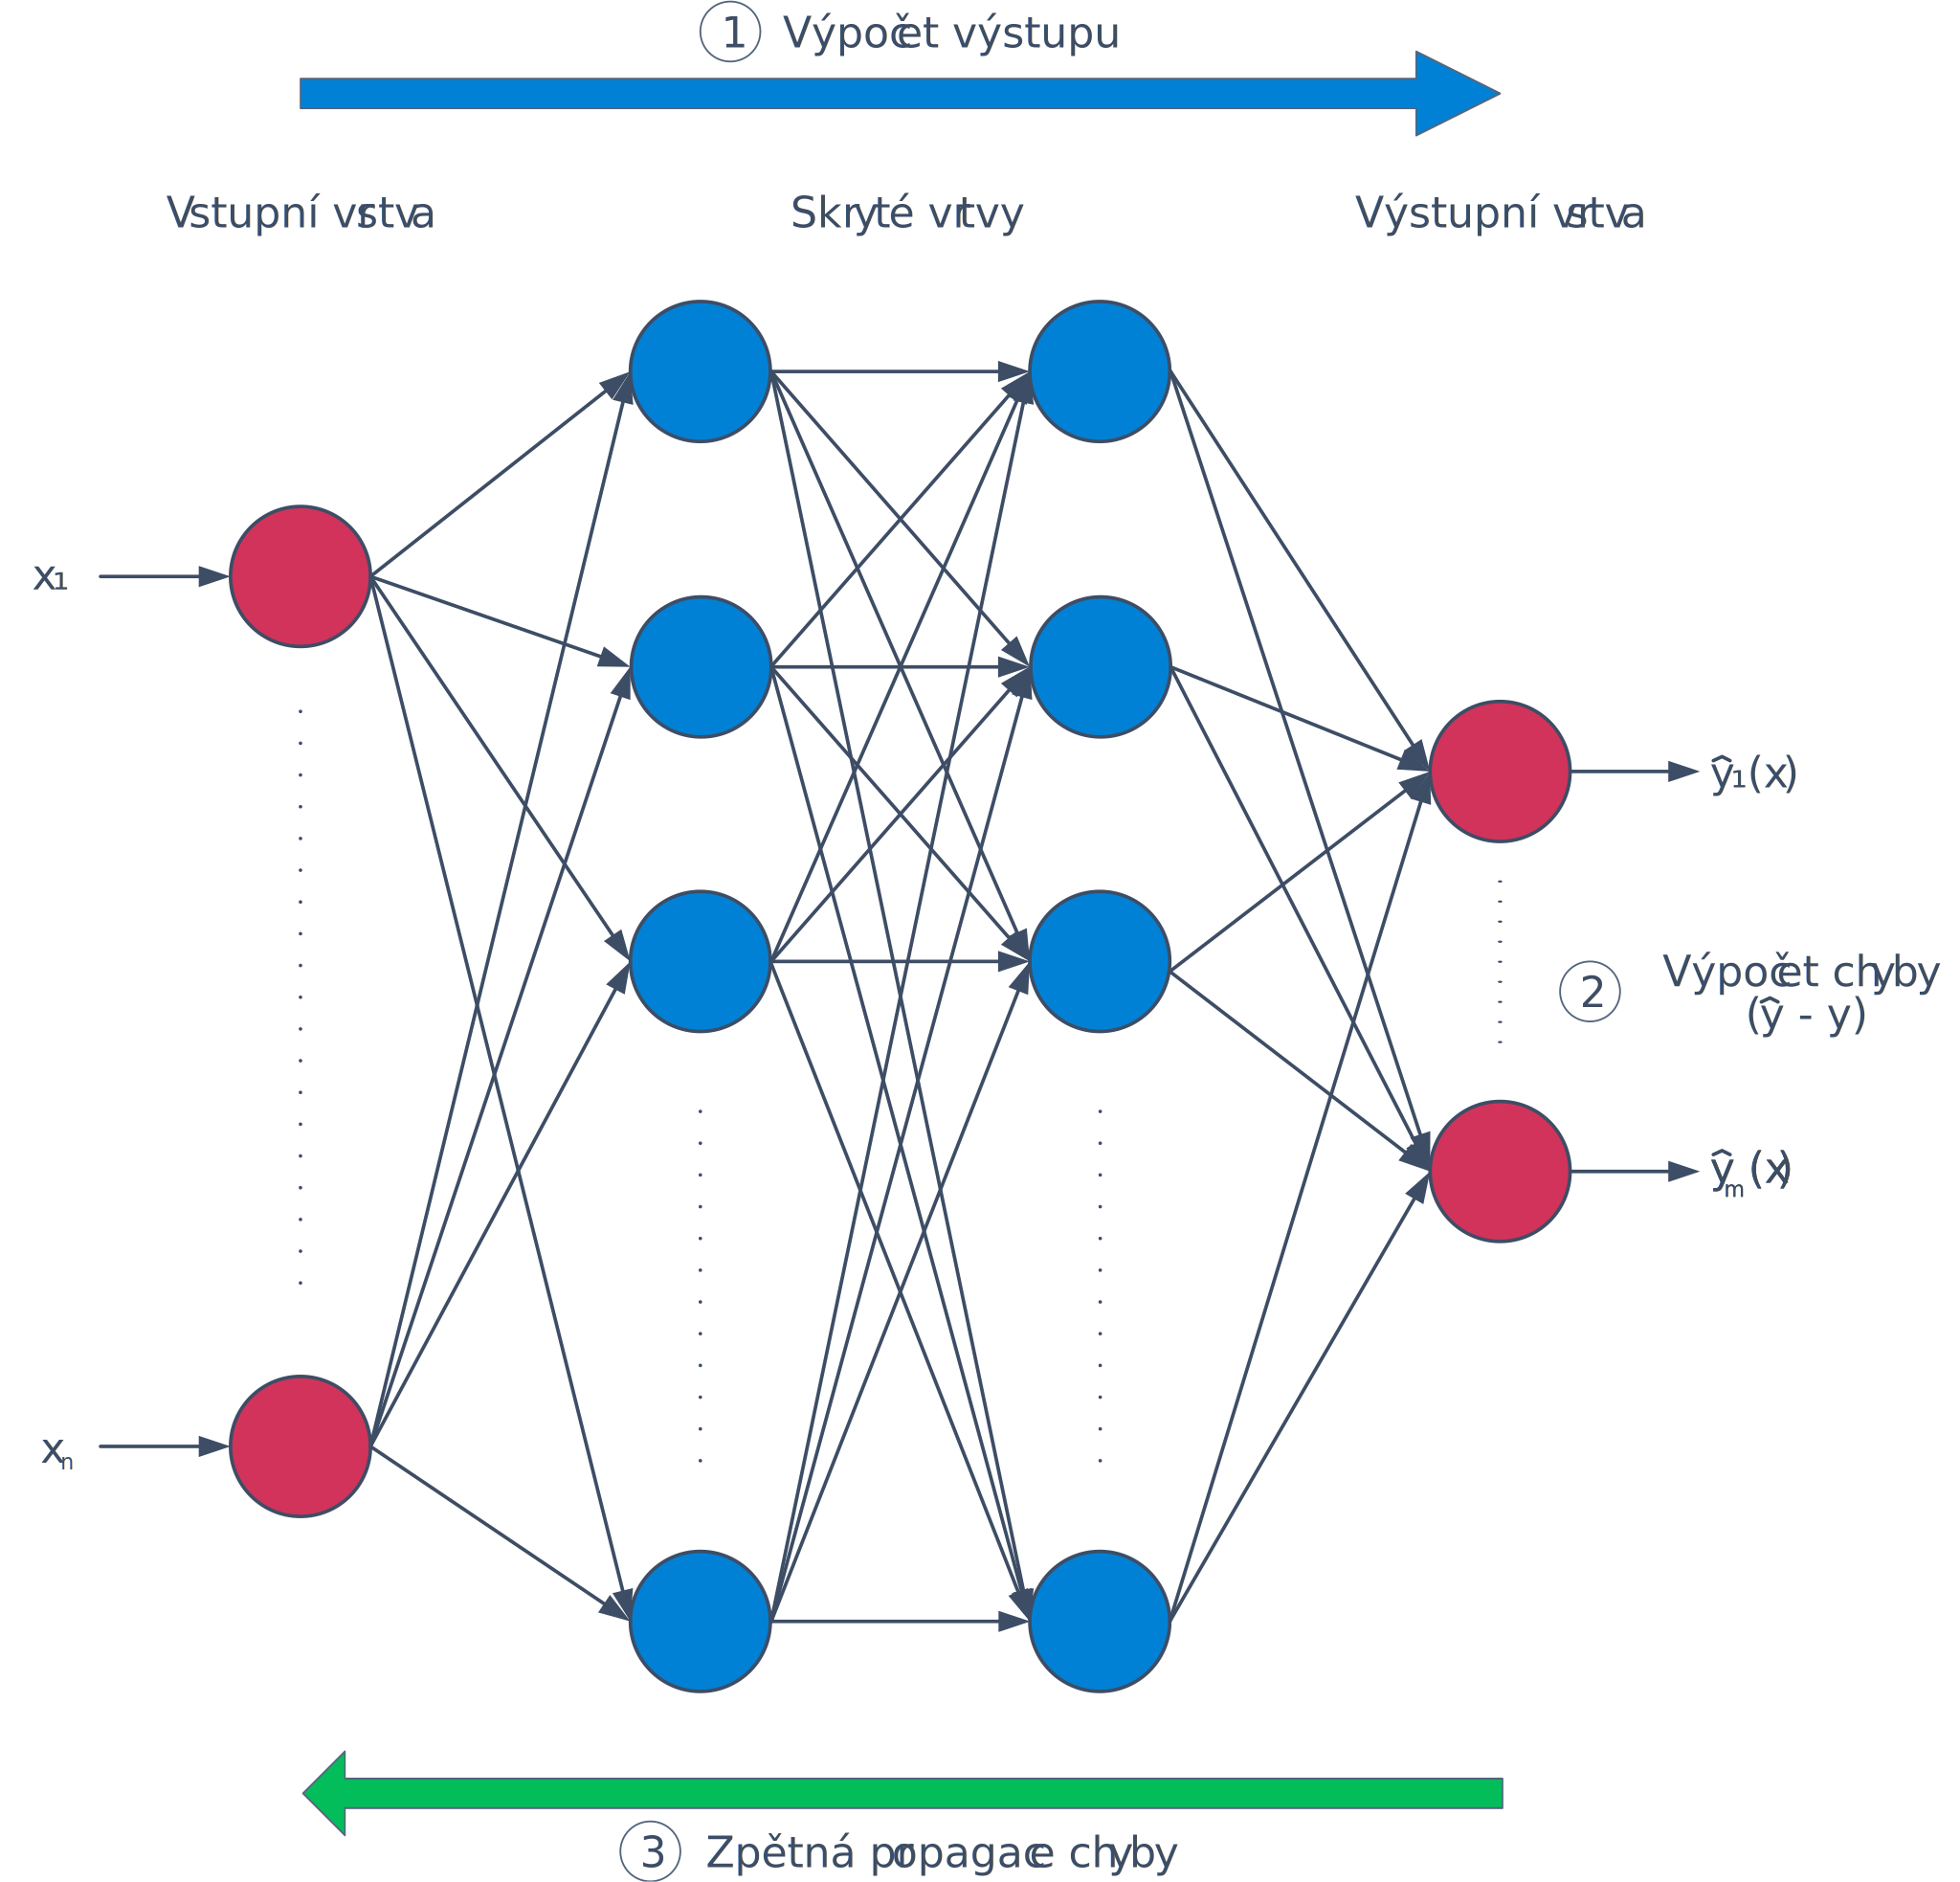
\includegraphics[width=0.9\textwidth]{./ch4-asr/img/dnn-training.pdf}
  \caption{Schéma a princip učení neuronové sítě.}
  \label{fig:asr:acoustic:dnn:training}
\end{figure}

Zmíněná aktivační funkce hraje velmi významnou roli, protože umožňuje řešení i problémů nelineárního charakteru. Pokud by NN nevyužívala aktivační funkce, jednalo by se de facto stále o lineární kombinaci vektorů, a tím pádem by bylo možné řešit jen lineární problémy. Mezi nejčastěji používané aktivační funkce patří \textit{sigmoid} ($\sigma\left(z\right) = \left(1 - e^{-z}\right)^{-1}$), \textit{tanh} ($\sigma\left(z\right) = \tanh\left(z\right)$) a \textit{relu} ($\sigma\left(z\right) = \max\left(0, z\right)$), jejich průběhy jsou ukázány na obr. \ref{fig:asr:acoustic:dnn:activation}.

 \begin{figure}[htpb]
  \centering
  \begin{subfigure}[b]{0.29\textwidth}
    \includegraphics[width=\textwidth]{./ch4-asr/img/sigmoid.png}
    \caption{sigmoid}
    \label{fig:asr:acoustic:dnn:activation:sigmoid}
  \end{subfigure}
  %
  \begin{subfigure}[b]{0.3\textwidth}
    \includegraphics[width=\textwidth]{./ch4-asr/img/tanh.png}
    \caption{tanh}
    \label{fig:asr:acoustic:dnn:activation:tanh}
  \end{subfigure}
  %
  \begin{subfigure}[b]{0.28\textwidth}
    \includegraphics[width=\textwidth]{./ch4-asr/img/relu.png}
    \caption{relu}
    \label{fig:asr:acoustic:dnn:activation:relu}
  \end{subfigure}
  \caption{Příklady používaných aktivačních funkcí.}
  \label{fig:asr:acoustic:dnn:activation}
\end{figure}

\newpage Pro výpočet výstupu $L$-vrstvé neuronové sítě je použit iterativní postup tzv. \textbf{forward propagation}, který lze matematicky zapsat jako

\begin{align}
  \begin{split}
    \mathbf{Z}^{[l]} = \mathbf{W}^{[l]}\mathbf{a}^{[l-1]} + \mathbf{b}^{[l]}, \\
    \mathbf{a}^{[l]} = \sigma^{[l]}\left(\mathbf{Z}^{[l]}\right),
  \end{split}
  \label{eq:asr:acoustic:dnn:fw}
\end{align}

\noindent kde $l = 1, \dots, L$, $\boldsymbol{a}^{[l]}$ představuje výstup $l$-té vrstvy ($\boldsymbol{a}^{[0]} = \boldsymbol{x}$), $\mathbf{W}^{[l]}$ představuje váhovou matici $l$-té vrstvy, $\mathbf{b}^{[l]}$ vektor prahů $l$-té vrstvy a $\sigma^{[l]}(.)$ aktivační funkci $l$-té vrstvy. Výsledkem iterativního výpočtu (\ref{eq:asr:acoustic:dnn:fw}) je výstup sítě $\hat{\boldsymbol{y}} = \boldsymbol{a}^{[L]}$.

Trénováním neuronové sítě je myšleno určení hodnot váhových matic $\mathbf{W}^{[l]}$ a prahů $\mathbf{b}^{[l]}$. Tento proces se iterativně sestává ze tří kroků (viz obr. \ref{fig:asr:acoustic:dnn:training})

\begin{enumerate}
  \item výpočet výstupu sítě dle vztahů (\ref{eq:asr:acoustic:dnn:fw});
  \item vypočtení chyby predikce $J\left(\boldsymbol{y}, \hat{\boldsymbol{y}}\right)$, kde $\boldsymbol{y}$ je učitel;
  \item aktualizace vah pomocí algoritmu backpropagation.
\end{enumerate}

\noindent Výpočet výstupu NN je realizován pomocí vztahů (\ref{eq:asr:acoustic:dnn:fw}). Následně je nezbytné vypočítat chybu predikce $J\left(\boldsymbol{y}, \hat{\boldsymbol{y}}\right)$ definovanou vztahem

\begin{equation}
  J\left(\boldsymbol{y}, \hat{\boldsymbol{y}}\right) = \frac{1}{M} \sum_{i=1}^{M}\mathcal{L}_{i}\left(\boldsymbol{y}^{i}, \hat{\boldsymbol{y}}^{i}\right),
  \label{eq:asr:acoustic:dnn:cost}
\end{equation}

\noindent kde $M$ je počet prvků trénovací množiny a $\mathcal{L}_{i}\left(\boldsymbol{y}^{i}, \hat{\boldsymbol{y}}^{i}\right)$ je funkce výpočtu chyby predikce $i$-tého prvku trénovací množiny. Podoba konkrétní funkce, pomocí níž je definována chyba predikce, závisí na typu řešené úlohy. Často se používá cross-entropie definována vztahem

\begin{equation}
  \mathcal{L}_{i}\left(\boldsymbol{y}^{i}, \hat{\boldsymbol{y}}^{i}\right) = - \sum_{j=1}^{m} y^{i}_{j} \log \hat{y}^{i}_{j},
  \label{eq:asr:acoustic:dnn:cost}
\end{equation}

\noindent kde $m$ je dimenze výstupního vektoru.

Samotná aktualizace parametrů sítě je realizována pomocí \textbf{backpropagation} algoritmem. Úlohou tohoto algoritmu je vypočtení parciálních derivací $\partial J / \partial \mathbf{W}^{[l]}$ a $\partial J/\partial \mathbf{b}^{[l]}$ pro všechny vrstvy sítě. Chyba predikce ve vrstvě $l$ je závislá na chybě v~předchozí vrstvě $l-1$, a tedy lze pro jejich vyjádření použít tzv. chain pravidlo. Parciální derivace pak mají následující podobu

\begin{align}
  \begin{split}
    \frac{\partial J}{\partial \mathbf{W}^{[l]}} & = \frac{\partial J}{\partial \mathbf{a}^{[l]}} \frac{\partial \mathbf{a}^{[l]}}{\partial \mathbf{z}^{[l]}} \frac{\partial \mathbf{z}^{[l]}}{\partial \mathbf{W}^{[l]}}, \\
    \frac{\partial J}{\partial \mathbf{b}^{[l]}} & = \frac{\partial J}{\partial \mathbf{a}^{[l]}} \frac{\partial \mathbf{a}^{[l]}}{\partial \mathbf{z}^{[l]}} \frac{\partial \mathbf{z}^{[l]}}{\partial \mathbf{b}^{[l]}}
  \end{split}
  \label{eq:asr:acoustic:dnn:partial}
\end{align}

\noindent Vztahy pro výpočet aktualizací parametrů sítě jsou pak následující

\begin{align}
  \begin{split}
    \delta^{[L]} & = \nabla_{a} J \odot \sigma'\left(\mathbf{z}^{[L]}\right), \\
    \delta^{[l]} & = \left(\left(w^{[l+1]}\right)^T \delta^{[l+1]}\right) \odot \sigma'\left(\mathbf{z}^{[l]}\right), \\
    \frac{\partial J}{\partial \mathbf{W}^{[l]}} & = \mathbf{a}^{[l-1]}\delta^{[l]}, \\
    \frac{\partial J}{\partial \mathbf{b}^{[l]}} & = \delta^{[l]},
  \end{split}
  \label{eq:asr:acoustic:dnn:bp}
\end{align}

\noindent kde $\nabla_a J = \partial J / \partial \mathbf{a}^{[L]}$ a $\odot$ představuje Hadamardův součin. Samotná aktualizace parametrů je realizována vztahy

\begin{align}
  \begin{split}
    \mathbf{W}^{[l]} & = \mathbf{W}^{[l]} - \alpha \frac{\partial J}{\partial \mathbf{W}^{[l]}}, \\
    \mathbf{b}^{[l]} & = \mathbf{b}^{[l]} - \alpha \frac{\partial J}{\partial \mathbf{b}^{[l]}},
  \end{split}
  \label{eq:asr:acoustic:dnn:update}
\end{align}

\noindent kde $\alpha$ reprezentuje koeficient učení.

\subsubsection{Spojení skrytých Markovových modelů a neuronových sítí}

Rozvoj výpočetní techniky, zejména GPU\footnote{Graphics Processing Unit} s~možností provádět obecné maticové operace, zapříčinil masivní využití tzv. hlubokých neuronových sítí (DNN). Ty se vyznačují vyšším počtem skrytých vrstev, což umožňuje řešit sofistikovanější problémy jako např. rozpoznávání souvislé řeči. Bohužel DNN end-to-end\footnote{Systém, který kompletně řeší rovnici (\ref{eq:asr:decoding:generic}) pomocí jediné DNN sítě. Tyto systémy jsou většinou postaveny na rekurentních neuronových sítích (RNN).} systém je zatím velmi komplikované vytvořit a provozovat zejména proto, že  k~úspěšnému natrénování je potřeba řádově více dat než u GMM \cite{Amodei2016}. Z tohoto důvodu jsou v~současné době nejčastěji využívané systémy postavené na kombinaci HMM a DNN (HMM-DNN). Rozdíl oproti end-to-end systému je v~tom, že cílem DNN není odhad $\hat{W}$, ale stejně jako v~případě HMM-GMM, určit rozdělení pravděpodobnosti $b_j\left(\boldsymbol{o}_t\right)$.

V případě HMM-GMM je odhad $b_j\left(\boldsymbol{o}_t\right)$ realizován Gaussovskými hustotními směsmi podle vztahu (\ref{eq:asr:acoustic:gmm:output}). Těchto směsí je tolik, kolik je unikátních stavů HMM. U DNN však žádné směsi  k~dispozici nejsou. Pokud je však výstupní vrstva typu \textbf{softmax}, jde výstup $j$-tého neuronu definován vztahem

\begin{equation}
  y_{j} = a_{j}^{[L]} = \frac{\mathsf{e}^{z_j}}{\sum_{i=1}^{m}\mathsf{e}^{z_i}},
  \label{eq:asr:acoustic:dnn:asr:softmax}
\end{equation}

\noindent a $m$ je počet neuronů v~poslední vrstvě, zároveň platí, že

\begin{equation}
  \sum_{j=1}^{m} y_{j} = 1.
  \label{eq:asr:acoustic:dnn:asr:softmax:criterium}
\end{equation}

\noindent Hodnoty složek, označené $y_{i}$, výstupního vektoru $\boldsymbol{y}$ mají pseudo-pravděpodobnostní charakter. Pokud tedy bude $m$ rovno počtu stavů HMM, pak výstupní pravděpodobnost $b_{j} \left(\boldsymbol{o}_t\right)$ pro emitující stav $j$ má, podle (\ref{eq:asr:acoustic:dnn:asr:softmax}) tvar

\begin{equation}
  b_{j} \left(\boldsymbol{o}_t\right) = y_{j} = \frac{\mathsf{e}^{z_j}}{\sum_{i=1}^{m}\mathsf{e}^{z_i}}.
  \label{eq:asr:acoustic:dnn:asr:softmax:criterium}
\end{equation}

\noindent Principiální rozdíl ve funkci HMM-GMM a HMM-DNN je znázorněn na obr. \ref{fig:asr:acoustic:dnn:asr:diff}.

\begin{figure}[htpb]
  \centering
  \begin{subfigure}[b]{0.4\textwidth}
    \includegraphics[width=\textwidth]{./ch4-asr/img/hmm-gmm.pdf}
    \caption{GMM}
    \label{fig:asr:acoustic:dnn:asr:diff:dnn}
  \end{subfigure}
  %
  \begin{subfigure}[b]{0.4\textwidth}
    \includegraphics[width=\textwidth]{./ch4-asr/img/hmm-dnn.pdf}
    \caption{DNN}
    \label{fig:asr:acoustic:dnn:asr:diff:dnn}
  \end{subfigure}
  \caption{Principiální rozdíl ve funkci GMM a DNN systému.}
  \label{fig:asr:acoustic:dnn:asr:diff}
\end{figure}

K natrénování DNN se používá zmíněného backpropagation algoritmu. V~poslední době se však prosadilo trénování využívající předtrénování DNN pomocí tzv. restricted Bolzmann machines (RBM) \cite{Hinton2012}. Předtrénování řeší problém, kdy se informace zpětně propagovaná pomocí backpropagation algoritmu úplně nepřenese zpět do počáteční vrstvy, protože gradient je příliš malý. Předtrénování pomocí RBM pomáhá lépe určit parametry sítě. Principiálně je tento proces znázorněn na obr. \ref{fig:asr:acoustic:dnn:pretraining}.

Nejprve je natrénován GRBM (Gaussian-Bernoulli RBM) model na minibatchích sestavených z mikrosegmentů řeči o konstantní délce, například $10\ ms$. Stav skrytých jednotek je použit  k~natrénování RBM. Tento proces se opakuje dokud není natrénován požadovaný počet vrstev výsledné sítě. Následně jsou jednotlivé RBM spojeny do deep belief sítě (DBN) a je přidána výstupní softmax vrstva dimenze rovné počtu HMM stavů (DBN-DNN). Tato DBN-DNN síť je pak diskriminativně trénována na základě zarovnání získaného pomocí HMM-GMM, více o tomto principu trénování v~\cite{Hinton2012} a \cite{Vesely2013}. Vstupem neuronové sítě je často mikrosegment $t$ a jeho okolní mikrosegmenty. Velmi často se používá okolí o rozsahu $t-2$ a $t+2$.

\begin{figure}[hbpt]
  \centering
  \includegraphics[width=0.9\textwidth]{./ch4-asr/img/pretraining.pdf}
  \caption[Princip předtrénování pomocí RBM.]{Princip předtrénování pomocí RBM s~třemi vrstvami \cite{Hinton2012}.}
  \label{fig:asr:acoustic:dnn:pretraining}
\end{figure}

\subsubsection{Time-delay neural networks}

Nevýhodou DNN sítí je, že pracují pouze se statickými parametry v~rámci zpracovávaných mikrosegmentů, protože sumace v~perceptronu odpovídá sumě vážených statických vstupů. Po zpracování mikrosegmentu $t$ není získaná informace nijak zohledněna při zpracování segmentu $t+1$. Tento nedostatek by řešilo použití rekurentních neuronových sítí (RNN). Bohužel tyto sítě mají mnohem komplikovanější buňku neuronu než FF sítě s~perceptronem \cite{Amodei2016}, proto je potřeba řádově více dat k~natrénování. Složitost buňky také zvyšuje komputační náročnost výpočtu \cite{Hannun2014}.

Dalším typem neuronových sítí jsou time-delay neural network (TDNN), které jsou podrobněji popsané v~\cite{Waibel1989}. Oproti výše popsaným NN je přidána časová filtrace do sumační části neuronu, tím je docíleno zahrnutí dynamické složky do výpočtu sítě \cite{Craig2000}. Filtrace je implementována jako filtr s~konečnou impulzní odezvou (FIR), tedy

\begin{equation}
  z_{j}^{[l]}\left(t\right) = \sum_{n=0}^{N} w_{j}^{[-n]}f\left(n\right)a^{[l-1]}_{j}\left(t - n\right) + b_{j},
  \label{eq:asr:acoustic:dnn:tdnn:fir}
\end{equation}

\noindent kde $t$ je diskrétní časový index, $N$ je délka FIR filtru, $f\left(n\right)$ odezva filtru v~bodě $n$, $w_{j}^{[-n]}$ příslušná váha, $a^{[l-1]}_{j}$ je výstup vrstvy $l-1$ a $z_{j}^{[l]}\left(t\right)$ je výstup sumační části neuronu $j$ ve vrstvě $l$. Vztah (\ref{eq:asr:acoustic:dnn:tdnn:fir}) tedy představuje konvoluci. Na obr. \ref{fig:asr:acoustic:dnn:tdnn:neuron} je principiálně znázorněn neuron pracující s~FIR filtrem $N$-tého řádu. Z obr. \ref{fig:asr:acoustic:dnn:tdnn:neuron} je také zřejmé, že TDNN síť má několik souborů vah $W^{x}$, které umožňují lépe pracovat s~dynamickou složkou signálu \cite{Peddinti2015}.

\begin{figure}[htpb]
  \centering
  \begin{subfigure}[b]{0.45\textwidth}
    \includegraphics[width=\textwidth]{./ch4-asr/img/neuron-tdnn.pdf}
    \caption{neuron}
    \label{fig:asr:acoustic:dnn:tdnn:neuron}
  \end{subfigure}
  %
  \begin{subfigure}[b]{0.35\textwidth}
    \includegraphics[width=\textwidth]{./ch4-asr/img/tdnn.pdf}
    \caption{síť}
    \label{fig:asr:acoustic:dnn:tdnn:net}
  \end{subfigure}
  \caption[Neuron TDNN sitě a její zjednodušené blokové schéma.]{Neuron TDNN sítě a zjednodušené blokové schéma TDNN sítě \cite{Craig2000}.}
  \label{fig:asr:acoustic:dnn:tdnn}
\end{figure}

Stejně jako v~případě DNN sítě je vstupem parametrizovaný mikrosegment $t$ a jeho okolí. Z obr. \ref{fig:asr:acoustic:dnn:tdnn:net} je patrné, že hlubší vrstvy postupně zpracovávají větší a větší okolí mikrosegmentu $t$. Dimenze výstupní vrstvy odpovídá počtu HMM stavů. Přestože je TDNN síť typu FF, tak dokáže pracovat i s~dynamickými parametry řeči, protože využívá princip konvoluce.
